\documentclass[a4paper]{report}

\usepackage[a4paper, total={6in, 10in}]{geometry}

\usepackage[utf8]{inputenc}
\usepackage{graphicx}
\usepackage{amsmath}
\usepackage{amsthm}
\usepackage{amssymb}
\usepackage{bbold}
\usepackage{tikz}
\usepackage{subcaption}
\usepackage[hidelinks]{hyperref}

\usetikzlibrary{positioning, quotes, arrows.meta, calc}

\theoremstyle{definition}
\newtheorem{theorem}{Theorem}[section]
\newtheorem{definition}{Definition}[section]
\newtheorem{corollary}{Corollary}[section]

\begin{document}

\title{Efficient instruction-level parallelism analysis using tropical semiring \lq{matrix multiplication\rq}}
\author{\small{ Bryan Abi Karam \textit{bca35@cam.ac.uk} }}
\maketitle

\tableofcontents

\chapter{Introduction} \label{chap:intro}

In my project, I...

\section{Instruction Level Parallelism}

\textit{Instruction level parallelism} is the simultaneous execution of instructions in a computer processor. These 
instructions come from a single specific thread of execution in a computer program, as opposed to 
concurrency, where instructions from many threads are executed concurrently, and therefore is known as
\textit{thread level parallelism}.

Theoretically, a pair of instructions from a single thread can be executed simultaneously when there exist no data 
dependencies between them. A data dependency between two instructions exists when the operation of the instruction
appearing later in the program order consumes a value that is produced by the operation of the instruction appearing 
before it in the program order (this is known as a read after write, or RaW dependency).

To avoid race conditions, which lead to unexpected or inconsistent results, a computer processor has to take these 
RaW dependencies into consideration when scheduling instructions for execution. An instruction dependent on a previous
one must be executed strictly after the former has produced its result, to ensure correct propagation of values in the 
program.

\subsection{Finding and exploiting ILP in processors}

Previously, processors were in-order and single issue, having a maximum IPC of 1. Each clock cycle, the processor would 
execute one instruction, in program order, usually through a pipelined architecture.
Modern processors commonly exploit ILP, through superscalar processing and out of order execution.
Superscalar processors issue several independent instructions in a single clock cycle, commonly exhibiting an IPC 
greater than 1. This means that instructions are scheduled and executed out of order, which is a technique also used
to hide latencies from complex operations and memory loads.

In fact, the absolute limit of the ILP a processor core can exploit is entirely dependent on the structure of 
the computer program it executes. The dynamic execution of a program will have a 'critical path', that is, a series of 
executed instructions, each data-dependent on the previous, that must be executed sequentially. A processor cannot execute 
the program faster than it can execute this critical path.

However, the amount of ILP a processor is able to find and exploit is usually lower than the theoretical limit, owing to 
hardware limitations. These can include:

\begin{itemize}
  \item Branch/jump mispredictions, which typically trigger a discard of all work after the point of misprediction.
  \item Stuctural hazards, such as busy functional units or slow memory accesses.
  \item The number of instructions a superscalar processor can issue at once.
  \item The size of the window used when looking for independent instructions to schedule.
  \item False data dependencies, known as Write-after-Write or Write-after-Read, which are a consequence of the limited 
    number of architectural registers. They are mitigated in hardware using register renaming to a larger set of physical
    registers hidden to the programmer, but ultimately we may not resolve all these hazards.
\end{itemize}

\section{ILP Limit Studies}

%TODO: CITATIONS??

Increasing the amount of ILP a processor can find and exploit is a crucial part of high-performance processor design,
and so studies are conducted to justify the effort put into this problem.

These studies look to measure the theoretical limit of exploitable ILP in a program, by measuring the length of its 
critical path. The maximum ILP available in a program is then the number of instructions executed in the dynamic 
execution of the program, divided by the length of the critical path.

\subsection{Methodology of limit studies}

Idealised models of program execution are commonly used to find the absolute maximum upper bound of ILP. The simulators 
are fed a trace of an actual program execution on real hardware or a functional simulator. Since this trace already 
provides the program's path of execution, the simulator does not need to compute the results of instructions, and so it
purely acts as a dependency graph analyser and critical path calculator.

Instructions have \textit{static} dependencies, where each individual instruction will read from and write to a fixed 
set of registers and memory locations at its execution. These dependencies for the whole program can be represented by 
its full dynamic dependency graph (DDG), which is a directed acyclic graph with one node per dynamically executed 
instruction in a program. The edges of the graph represent dependencies between dynamically executed instructions,
and so the length of the critical path is the length of the longest path through the program's DDG.

% TODO: include diagram for DDG?

Limit studies will also vary the parameters of the analysis, using perfect models that ignore all hardware restrictions
and try to find the theoretical limit of ILP available in a program, or instead introducing realistic bounds, such as
control flow models (imperfect branch prediction), and instruction window scaling, where ILP is only computed within a
smaller window of instructions (instead of the whole program), to identify how 'local' a program's ILP is.

\section{Motivations}

% Why do we want to develop a new methodology for limit studies?

%TODO: SOURCE??

Traditionally, simulation models use an algorithm that iterates over the execution trace, and at each step calculates 
the length of dependency paths ending at each register, eventually picking out the longest path at the end of the trace.
Because the dynamic trace inherently guarantees that a producer instruction appears before its consumer,
the trace acts as a topological sort of the DDG. Therefore, starting at the first instruction in the trace,
the algorithm amounts to a single-pass linear sweep over this topologically sorted graph to calculate the longest path.

The weakness of this approach is that the traversal of the topological sort of the DDG is inherently sequential and 
this makes it unscalable for traces containing trillions of instructions. It cannot be heavily parallelised, nor can it 
exploit memoisation of repetitions in program stucture such as loops.

%TODO: CITATION

To break this sequential bottleneck, Chadwick proposes a matrix-based approach. The idea is to represent the dependencies 
between each two instructions in the trace as a matrix, and use matrix multiplication in the max-tropical semiring to 
compute the longest path in the DDG. This approach becomes a problem of reducing a large expression of matrix multiplications.

The immediately obvious benefit is that the matrix expression is a divisible computation, due to the associativity of 
matrix multiplication. The multiplications can be carried out in any order, and intermediate results fully encode the
dependency information of the instructions they range over. This enables a range of optimisations, including
thread-level parallelisation, result memoisation, and order of operations based on heuristics.

One additional benefit of the divisibility of the matrix expression is that it makes instruction window scaling for 
limit studies much easier. Consider three windows of instructions: A, B, and C (which is comprised of windows A and B
consecutively). To compute ILP information for each window, the traditional approach must be executed 3 times, once for 
each window. However, the matrix-based approach will only need to run twice, on A and B, and the dependency 
information matrix for C can simply be obtained by multiplying the result matrices from A and B.

In this project, I will explore several approaches for performing Chadwick's matrix-based approach efficiently, 
considering various types of parallelism, including at the data, thread, and accelerator level. I will then benchmark 
and evaluate these approaches, demonstrating a performance improvement over the 'classical' technique for computing 
dependency chains.

\chapter{Preparation}

\section{Understanding the matrix-based approach}

\textit{The following applications of tropical semirings to dynamic dependency graphs, particularly the sections on 
alternative graph structures (\ref{chap:prep:alternative-graph-structure})
and register-only longest chains (\ref{chap:intro:section:register-only-chains})
are closely adapted from the methodologies established by Chadwick \cite{Chadderz}.}

\subsection{The tropical semiring (max-plus algebra)}

Tropical analysis is a branch of pure mathematics that is the study of the tropical semiring.
There are two variants of the tropical semiring, namely the min-plus and max-plus algebras.
We will use the max-plus convention to apply to \textit{longest} paths in directed acyclic graphs.

 
% Define tropical semiring and operations 

\begin{definition}[Semiring] \label{def:semiring}
  A semiring \cite{Wandsnider2020} is a set $R$ along with two operations, addition (+) and multiplication ($\cdot$), which satisfy the 
  following axioms:

  \begin{enumerate}
    \item Addition is associative and commutative.
    \item Multiplication is associative.
    \item There exists an additive identity, which we usually call $\mathbb{0}$. Additionally, $\mathbb{0}$ annihilates 
      $R$, that is, for all $x \in R$, $\mathbb{0} \cdot x = x \cdot \mathbb{0} = \mathbb{0}$.
    \item There exists a multiplicative identity, which we usually call $\mathbb{1}$.
    \item Multiplication left and right distributes over addition.
  \end{enumerate}
\end{definition}

\begin{definition}[Tropical semiring]
  The tropical semiring \cite{Wandsnider2020}, or max-plus algebra, is the object $(\mathbb{R} \cup \{-\infty\}, \oplus, \odot)$ with operations 
defined as:

$$
\begin{aligned}
  a\oplus b &= \max(a,b) \\
  a\odot b &= a+b
\end{aligned}
$$

\end{definition}

The tropical semiring satisfies the axioms of a semiring from Definition \ref{def:semiring}. It
is not a ring as the max operator does not have an inverse.

% Define matrix multiplication in the context of the tropical semiring

\begin{definition}[Matrix operations in the tropical semiring]
For any $n\times n$ matrices $X = (x_{ij})$ and $Y = (y_{ij})$, the entries of $U = X \oplus Y$ and $V = X \odot Y$
are calculated as \cite{krivulin2012maxplusalgebraapproachmodelling}

$$
u_{ij} = x_{ij} \oplus y_{ij}, \text{ and } v_{ij} = \displaystyle\sum_{k=1}^{n} \! {}_{\oplus} x_{ik} \odot y_{kj}
$$

\end{definition}

The matrix operations $\oplus$ and $\odot$ are associative owing to the commutativity and associativity of the underlying 
addition operator, and that the multiplication operator distributes over addition.

\subsection{Longest paths in Directed Acyclic Graphs}


% Show how this applies to the longest-path problem

As established previously, finding the length of the critical path in a program amounts to finding the longest path
in its DDG. It is noted that the max-plus version of the tropical semiring is applicable to finding the longest path
in a graph.

One algorithm to find the longest path between nodes $A$ and $B$ in a graph is to recursively take the 
maximum of all path lengths from all neighbours of $A$ to $B$, plus the cost of the edge from $A$ to the chosen
neighbour. We can see that this amounts to a Bellman recursion equation \cite{Bellman:DynamicProgramming}
involving only the max and plus operators: 

$$
v(A,B) = 
\begin{cases}
0 &\text{ if } A = B \\
\max_{\forall C . A \to C} \{\mathrm{weight}(A \to C) + v(C,B))\}, &\text{ otherwise } \\
\end{cases}
$$

We can observe that, if we have an adjacency matrix (where the cells in that matrix represent the cost of the edge
between the pair of nodes in that row/column, and $-\infty$ if there is no edge), performing tropical semiring 
matrix multiplication of this matrix with itself corresponds to one step of our longest-path algorithm.

Consider an adjacency matrix $X^{2} = X \odot X$, and denote its entries by $x_{ij}^{(2)}$. We have that $x_{ij}^{(2)} = p$
if and only if there exists at least one path of length $p$ from node $i$ to node $j$ in the corresponding graph,
consisting of at most two edges, and that path is the longest such path. This extends to any integer exponent $q$.

\begin{theorem}[Matrix exponentiation results in longest paths] \label{thm:mat-exp-longest-paths}

For any integer $q>0$, the matrix
$X^{q}$ has the entry $x_{ij}^{(q)} = p$ only if there is a path of length $p$ with at most $q$ edges from $i$ to $j$,
and that path is the longest such path. \cite{krivulin2012maxplusalgebraapproachmodelling}.

\begin{proof}
  We proceed by induction on $q$, the maximum number of edges in the path.

  \textbf{Base case ($q = 1$):} Consider the matrix $X^1=X$. By the definition of an adjacency matrix, the entry  
  $x_{ij}^{(1)}$ is exactly the weight of the direct edge from node $i$ to node $j$. If no such edge exists, then 
  $x_{ij}^{(1)} = -\infty$. Thus, the base case holds: the entries represent their longest paths consisting of at most 
  one edge.

  \textbf{Inductive step:} Assume the claim holds for $q$. That is the matrix $X^{q}$ has entries $x_{ij}^{q}$ 
  representing the longest path from $i$ to $j$ using at most $q$ edges.
  We show that the claim holds for $q+1$. By definition, $X^{q+1} = X^{q} \odot X$
  The entry $x_{ij}^{(q+1)}$ is calculated as:
  $$x_{ij}^{(q+1)} = \sum_{k=1}^{n} \! {}_{\oplus} (x_{ik}^{(q)}\odot x_{kj})$$
  Translating this to the original operators:
  $$
  x_{ij}^{(q+1)} = \max_{1 \leq k \leq n} (x_{ik}^{(q)} + x_{kj})
  $$
  This lines up perfectly with the dynamic programming approach to finding the longest path. To find a longest path from
  node $i$ to node $j$, it checks every intermediate node $k$. It takes the longest known path from $i$ to $k$ of at most 
  $q$ edges (by the inductive hypothesis), and adds the direct edge cost from $k$ to $j$. By taking the maximum over all 
  intermediate nodes $k$, we find the absolute longest path from $i$ to $j$ of at most $q+1$ edges. Thus the claim holds 
  for all integers $q>0$.
\end{proof}

So, an adjacency matrix raised to the power infinity will converge to the longest distance matrix for that whole graph.
  
\end{theorem}


For example, consider the graph:
\begin{center}
\begin{tikzpicture}[
    node distance=1cm and 2cm, % vertical and horizontal spacing
    every node/.style={font=\Large} % makes letters look like your image
]
    % Place the nodes
    \node (a) {a};
    \node (b) [right=of a] {b};
    \node (c) [below=of b] {c};
    \node (d) [right=of c] {d};

    % Draw the edges (undirected lines) with labels
    \draw [->] (a) -- node[above] {1} (b);
    \draw [->] (a) -- node[below left] {3} (c);
    \draw [->] (b) -- node[right] {1} (c);
    \draw [->] (c) -- node[above] {1} (d);
\end{tikzpicture}
\end{center}

The corresponding adjacency matrix would be:
$$
X = 
\begin{pmatrix}
  0 & 1 & 3 & -\infty \\ 
  -\infty & 0 & 1 & -\infty \\ 
  -\infty & -\infty & 0 & 1 \\
  -\infty & -\infty & -\infty & 0 \\
\end{pmatrix}
$$

So, in the tropical semiring:

$$
\begin{aligned}
  X^{2} &= 
  \begin{pmatrix}
    0
  \end{pmatrix} \\ 
  X^{3} &= 
  \begin{pmatrix}
    0
  \end{pmatrix}
\end{aligned}
$$

\subsection{Forming the DDG and register-only longest chains} \label{chap:intro:section:register-only-chains}

TODO

\subsection{Alternative graph structure} \label{chap:prep:alternative-graph-structure}

% Show how we arrange the DDG such that we can have a matrix representing dependencies of an instr.

Dynamic dependency graphs typically exhibit a layered, sequential structure - they are more long than wide. While a 
standard $N \times N$ adjacency matrix (where $N$ is the total number of dynamically executed instructions) could 
map the graph, it is inefficient.
This is because, in the DDG, edges \textit{only} 
exist between adjacent columns. Therefore, the full adjacency matrix $X$ is mostly filled with $-\infty$.
Instead, the DDG can be modelled as a sequence of adjacent columns. 
Consider an arbitrary graph with the property of being more long than wide:

\begin{center}
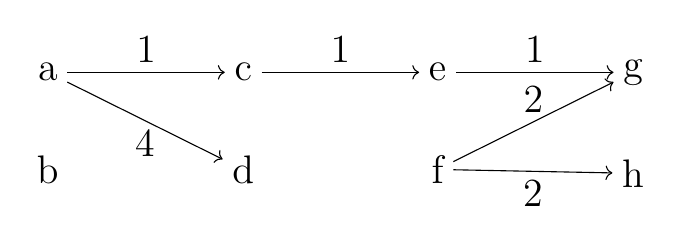
\begin{tikzpicture}[
    node distance=0.7cm and 2cm, % vertical and horizontal spacing
    every node/.style={font=\Large} % makes letters look like your image
]
    % Place the nodes
    \node (a) {a};
    \node (b) [below=of a] {b};
    \node (c) [right=of a] {c};
    \node (d) [below=of c] {d};
    \node (e) [right=of c] {e};
    \node (g) [right=of e] {g};
    \node (f) [below=of e] {f};
    \node (h) [below=of g] {h};

    % Draw the edges (undirected lines) with labels
    \draw [->] (a) -- node[above] {1} (c);
    \draw [->] (a) -- node[below] {4} (d);
    \draw [->] (c) -- node[above] {1} (e);
    \draw [->] (e) -- node[above] {1} (g);
    \draw [->] (f) -- node[above] {2} (g);
    \draw [->] (f) -- node[below] {2} (h);
\end{tikzpicture}
\end{center}

Whilst we could use the adjacency matrix representation, the structure lends itself to another representation for 
longest path problems. First of all, we modify the graph such that the longest path will always connected to the 
rightmost part of the graph, by adding extra nodes and cost-0 edges, and so also each path is connected to the first 
column similarly.

To utilize column-wise matrices for longest-path calculations, the graph must first be padded. We introduce a set of 
'dummy' nodes to the first and last columns, connected by 0-cost edges. This guarantees that any local path within the 
interior of the graph is extended to touch both the initial and final columns.

\begin{center}
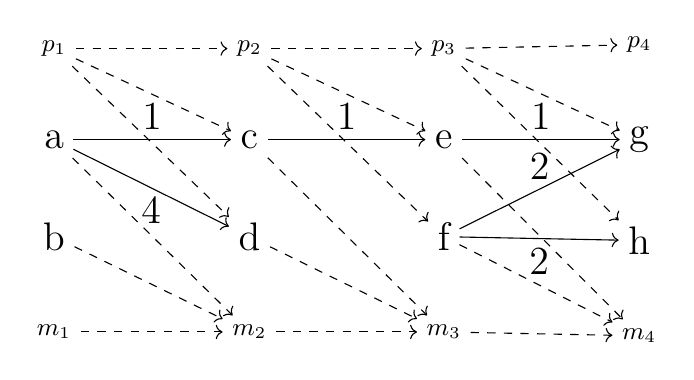
\begin{tikzpicture}[
    node distance=0.7cm and 2cm, % vertical and horizontal spacing
    every node/.style={font=\Large} % makes letters look like your image
]
    % Place the nodes
    \node (a) {a};
    \node (b) [below=of a] {b};
    \node (c) [right=of a] {c};
    \node (d) [below=of c] {d};
    \node (e) [right=of c] {e};
    \node (g) [right=of e] {g};
    \node (f) [below=of e] {f};
    \node (h) [below=of g] {h};

    \node (p1) [above=of a, font=\small] {$p_1$};
    \node (p2) [above=of c, font=\small] {$p_2$};
    \node (p3) [above=of e, font=\small] {$p_3$};
    \node (p4) [above=of g, font=\small] {$p_4$};

    \node (m1) [below=of b, font=\small] {$m_1$};
    \node (m2) [below=of d, font=\small] {$m_2$};
    \node (m3) [below=of f, font=\small] {$m_3$};
    \node (m4) [below=of h, font=\small] {$m_4$};

    % Draw the edges with labels
    \draw [->] (a) -- node[above] {1} (c);
    \draw [->] (a) -- node[below] {4} (d);
    \draw [->] (c) -- node[above] {1} (e);
    \draw [->] (e) -- node[above] {1} (g);
    \draw [->] (f) -- node[above] {2} (g);
    \draw [->] (f) -- node[below] {2} (h);

    % draw the zero-cost edges
    \draw [->, dashed] (p1) -- (p2);
    \draw [->, dashed] (p1) -- (c);
    \draw [->, dashed] (p1) -- (d);

    \draw [->, dashed] (p2) -- (p3);
    \draw [->, dashed] (p2) -- (e);
    \draw [->, dashed] (p2) -- (f);

    \draw [->, dashed] (p3) -- (p4);
    \draw [->, dashed] (p3) -- (g);
    \draw [->, dashed] (p3) -- (h);

    \draw [->, dashed] (a) -- (m2);
    \draw [->, dashed] (b) -- (m2);
    \draw [->, dashed] (m1) -- (m2);

    \draw [->, dashed] (c) -- (m3);
    \draw [->, dashed] (d) -- (m3);
    \draw [->, dashed] (m2) -- (m3);

    \draw [->, dashed] (e) -- (m4);
    \draw [->, dashed] (f) -- (m4);
    \draw [->, dashed] (m3) -- (m4);
\end{tikzpicture}

{\tiny dashed edges are 0 cost}
\end{center}

Now we can represent the graph with one matrix per adjacent-column pair, encoding the connectivity between those two
columns. The connectivity between the first two columns is represented as:

\[
  X_{1,2} = 
  \begin{pmatrix}
  0 & 0 & 0 & -\infty \\
  -\infty & 1 & 4 & 0 \\
  -\infty & -\infty & -\infty & 0 \\
  -\infty & -\infty & -\infty & 0 
  \end{pmatrix}
\]

where the $m$th row and $n$th column of this matrix represent the connection from the $m$th node in the first column of 
the graph to the $n$ node in the second column of the graph.

The remaining two column pairs are represented as:

\[
  \begin{aligned}
    X_{2,3} &= 
    \begin{pmatrix}
    0 & 0 & 0 & -\infty \\
    -\infty & 1 & -\infty & 0 \\
    -\infty & -\infty & -\infty & 0 \\
    -\infty & -\infty & -\infty & 0 
    \end{pmatrix} \\
    X_{3,4} &= 
    \begin{pmatrix}
    0 & 0 & 0 & -\infty \\
    -\infty & 1 & -\infty & 0 \\
    -\infty & 2 & 2 & 0 \\
    -\infty & -\infty & -\infty & 0 
    \end{pmatrix}\\
  \end{aligned}
\]

These matrices are each $4 \times 4$ whereas a full adjacency matrix for the original graph would be $7 \times 7$.
We can see that the column-wise matrices will use less storage than the adjacency matrix (48 integers vs 49 integers),
and this alternative becomes increasingly favourable as the graph gets longer.


In the tropical semiring, computing the matrix product

\[
  X_{3,4} \odot X_{2,3} \odot X_{1,2} = \begin{pmatrix}
  0 & 2 & 2 & 1 \\
  -\infty & 3 & -\infty & 4 \\
  -\infty & -\infty & -\infty & 0 \\
  -\infty & -\infty & -\infty & 0 
\end{pmatrix}
\]
yields a matrix representing the longest path from the $m$th node in the first column the $n$th node in the final 
column of the graph. Because we have ensured every path in the graph connects to the first and last column, the largest 
individual value in this matrix is the length of the longest path in the graph, namely the path of length 4 connecting 
from $a$ in the first column, to $m_4$ in the final column, via $d$ and $m_3$.

The correctness of the column-wise approach for calculating longest paths in graphs is a corollary that follows directly 
from Theorem \ref{thm:mat-exp-longest-paths}.

\begin{corollary}[Correctness of the column-wise formulation]
  In a standard adjacency matrix $X$, computing $X^{q}$ checks every possible intermediate node 
  $k$ in the entire graph to find paths of length $q$, as shown by Theorem \ref{thm:mat-exp-longest-paths}.

  In the DDG, when we multiply adjacent column matrices (e.g., $X_{2,3} \odot X_{1,2}$),
  we are simply performing the exact operations for finding the longest path between columns 1 and 3,
  but restricted only to the intermediate nodes $k$ located in column $2$.
  This is valid as edges in the DDG only exist between adjacent columns.

  Because the padding of 0 cost edges ensures every path spans from the first column to the final column, multiplying 
  all consecutive column matrices sequentially computes the maximum path length across the entire graph.
\end{corollary}

This defines the shape of the data will be working on. 

\section{Datasets}

\include{sections/3-impl}
\include{sections/4-eval}
\include{sections/5-conc}

\bibliography{references}{}
\bibliographystyle{plain}

\end{document}
